\documentclass{beamer}
\usetheme{Berlin}
\usefonttheme{serif}

\setbeamercolor{frametitle}{bg=black,fg=white}
\setbeamercolor{title}{bg=black,fg=white}
\setbeamercolor{section in head/foot}{bg=brown,fg=white}
\setbeamercolor{subsection in head/foot}{bg=brown,fg=white}
\setbeamercolor{navigation symbols}{fg=brown}
\setbeamercolor{normal text}{fg=black}

\fontsize{14}{16}\selectfont
\fontseries{b}\selectfont

\usepackage{fbox}
\setlength{\fboxrule}{1pt}
\setlength{\fboxsep}{0pt}

\usepackage{shadow}

\title{WordVerse} 
\subtitle{}
\author{\bfseries Sheetal Lodhi \and \bfseries Sonakshi Raj }
\date{\today}

\begin{document}
 
\begin{frame}
    \titlepage
\end{frame}

\section{Introduction}

\begin{frame}{\bfseries Introduction}
    \begin{itemize}
        \item \bfseries WordVerse is a web application designed for playing the Wordle game.
        \item \bfseries We've got two awesome modes for you: 'Guess My Word' where you try to figure out a mystery word, and 'I'll Guess Yours' where our chatbot tries to read your mind
    \end{itemize}
\end{frame}

\section{Project Motivation}

\begin{frame}{\bfseries Why WordVerse?}
    \begin{itemize}
        \item \bfseries WordVerse is an interactive game that requires real-time communication between the client and server. This makes it an ideal project for learning WebSockets, which enable bi-directional communication between the client and server
        \item \bfseries It offers us a opportunity to learn golang. 
    \end{itemize}
\end{frame}

\section{Key Features}

\begin{frame}{\bfseries Key Features of WordVerse}
    \begin{itemize}
        \item \bfseries Classic Wordle game.
        \item \bfseries NPC Character (bot) that interacts with users and assists in gameplay.
        \item \bfseries Responsive design optimized for different devices.
        \item \bfseries Real-time communication using WebSocket.
        \item \bfseries Backend implemented in Go.
        \item \bfseries User-selected secret word functionality.
    \end{itemize}
\end{frame}

\section{Technologies Used}

\begin{frame}{\bfseries Technologies and Tools}
    \begin{itemize}
        \item \bfseries Frontend: React, CSS.
        \item \bfseries Backend: Go, WebSocket.
        \item \bfseries Libraries: LaTeX, Gin.
    \end{itemize}
\end{frame}

\section{Challenges}

\begin{frame}{\bfseries Challenges we have faced}
    \begin{enumerate}
        \item \bfseries Chatbot response handling.
        \item \bfseries Setting up React was a major pain point.
        \item \bfseries Implementing Gorilla Websocket.
        \item \bfseries Major challenge - Fixing one bug would often trigger another. 
        \item \bfseries Balancing college and project life
        
    \end{enumerate}
\end{frame}

\section{Our Learnings So Far}

\begin{frame}{\bfseries Our Learnings So Far}
    \begin{enumerate}
        \item \bfseries Teamwork 
        \item \bfseries Error solving
        \item \bfseries Go 
        \item \bfseries CLI: Mastered navigating command lines for efficient workflow. 
        \item \bfseries Gorilla Websocket
        \item \bfseries Frontend tech: Learned HTML, CSS, JavaScript for UI building 
        \item \bfseries React
        
    \end{enumerate}
\end{frame}

\section{Proud Achievements}

\begin{frame}{\bfseries Proud Moments}
    \begin{itemize}
        \item \bfseries Custom-built NPC character (bot) with unique interaction logic.
        \item \bfseries Efficient and clean file structure that made the project easy to manage.
        \item \bfseries Successfully implementing real-time communication, enhancing user interaction.
        \item \bfseries The successful deployment of the project and the positive feedback received.
    \end{itemize}
\end{frame}

\section{Project Timeline}

\begin{frame}{\bfseries Project Timeline}
    \begin{itemize}
        \item \bfseries Week 1-2: Project planning and research
        \item \bfseries Week 3-4: Frontend development
        \item \bfseries Week 5-6: Backend development
        \item \bfseries Week 7-8: Testing and debugging
        \item \bfseries Week 9: Deployment and feedback
    \end{itemize}
\end{frame}

\section{File Structure Overview}
\begin{frame}{\bfseries Understanding the File Structure}
    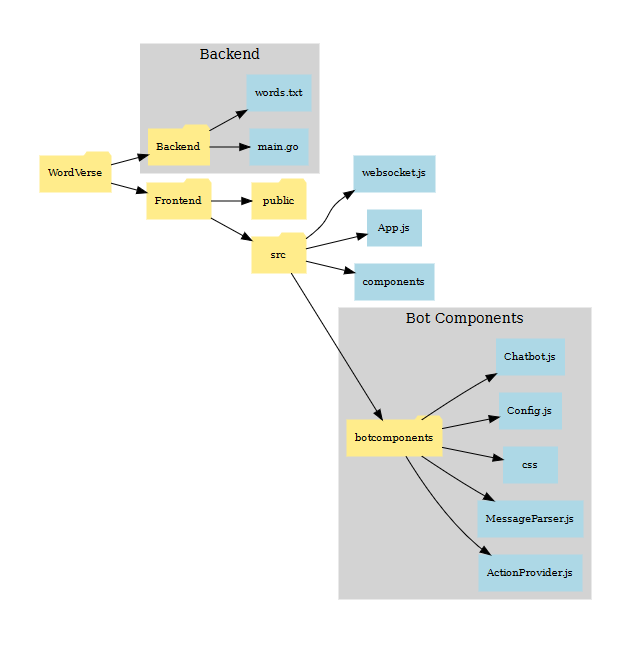
\includegraphics[scale=0.4]{struc.png}
\end{frame}

\section{References}

\begin{frame}{\bfseries References}
    \begin{itemize}
        \item \bfseries For Go: \url{https://go.dev/doc/}
        \item \bfseries For Gin: \url{https://gin-gonic.com/docs/}
        \item \bfseries For WebSocket: \url{https://websockets.readthedocs.io/en/stable/index.html}
        \item \bfseries For React: \url{https://react.dev/}
        \item \bfseries Postman API Documentation: \url{https://www.postman.com/api-platform/api-documentation/}
    \end{itemize}
\end{frame}

\begin{frame}
    \begin{center}
        \LARGE
        \shadowtext{\bfseries Thank You}
    \end{center}
\end{frame}

\end{document}